\chapter{Implementation}

This chapter explains how the design described in Chapter 3 was implemented in the project. The purpose of this chapter is not to document every source file or every function, but to show how the main architectural decisions were turned into a working system.

\section{Implementation Overview}

The implementation is divided into four main parts: the Qt/QML graphical application, the host-side controller, the firmware communication layer, and the vault manager. The QML layer presents the user workflows. The \texttt{VaultController} class coordinates state and operations. The \texttt{SerialBridge} class communicates with the STM32 firmware over USB-UART. The \texttt{vault\_manager} program performs system-level storage operations.

\begin{table}[!htbp]
\centering
\caption{\label{tab:implementation-units}Main implementation units.}
\small
\begin{tabularx}{\textwidth}{lXX}
\toprule
Unit & Main files & Role in the project\\
\midrule
GUI layer & QML screens & Presents vault setup, detail, lock/unlock, logs, and settings workflows\\
Host controller & \texttt{vault\_controller.cpp} & Coordinates state, validation, registry, logs, and asynchronous operations\\
Serial bridge & \texttt{serial\_bridge.cpp} & Sends firmware commands and receives fingerprint/key responses\\
Vault manager & \texttt{vault\_manager.c} & Creates encrypted containers and performs mount, unmount, loop-device, and cleanup operations\\
\bottomrule
\end{tabularx}
\end{table}

With this split, the user interface stays simple and disk operations are not placed directly inside QML. The GUI asks for an operation, the controller checks the current state, and the vault manager performs the storage action when needed.

\section{Physical Prototype}

The hardware prototype connects the AS608 fingerprint sensor to the STM32 Blue Pill, and the STM32 communicates with the host computer through the PL2303 USB-UART bridge. The physical setup was used during firmware communication tests, fingerprint enrollment and verification tests, and complete vault workflow tests.

\begin{figure}[!htbp]
    \centering
    \begin{minipage}[t]{0.48\textwidth}
        \centering
        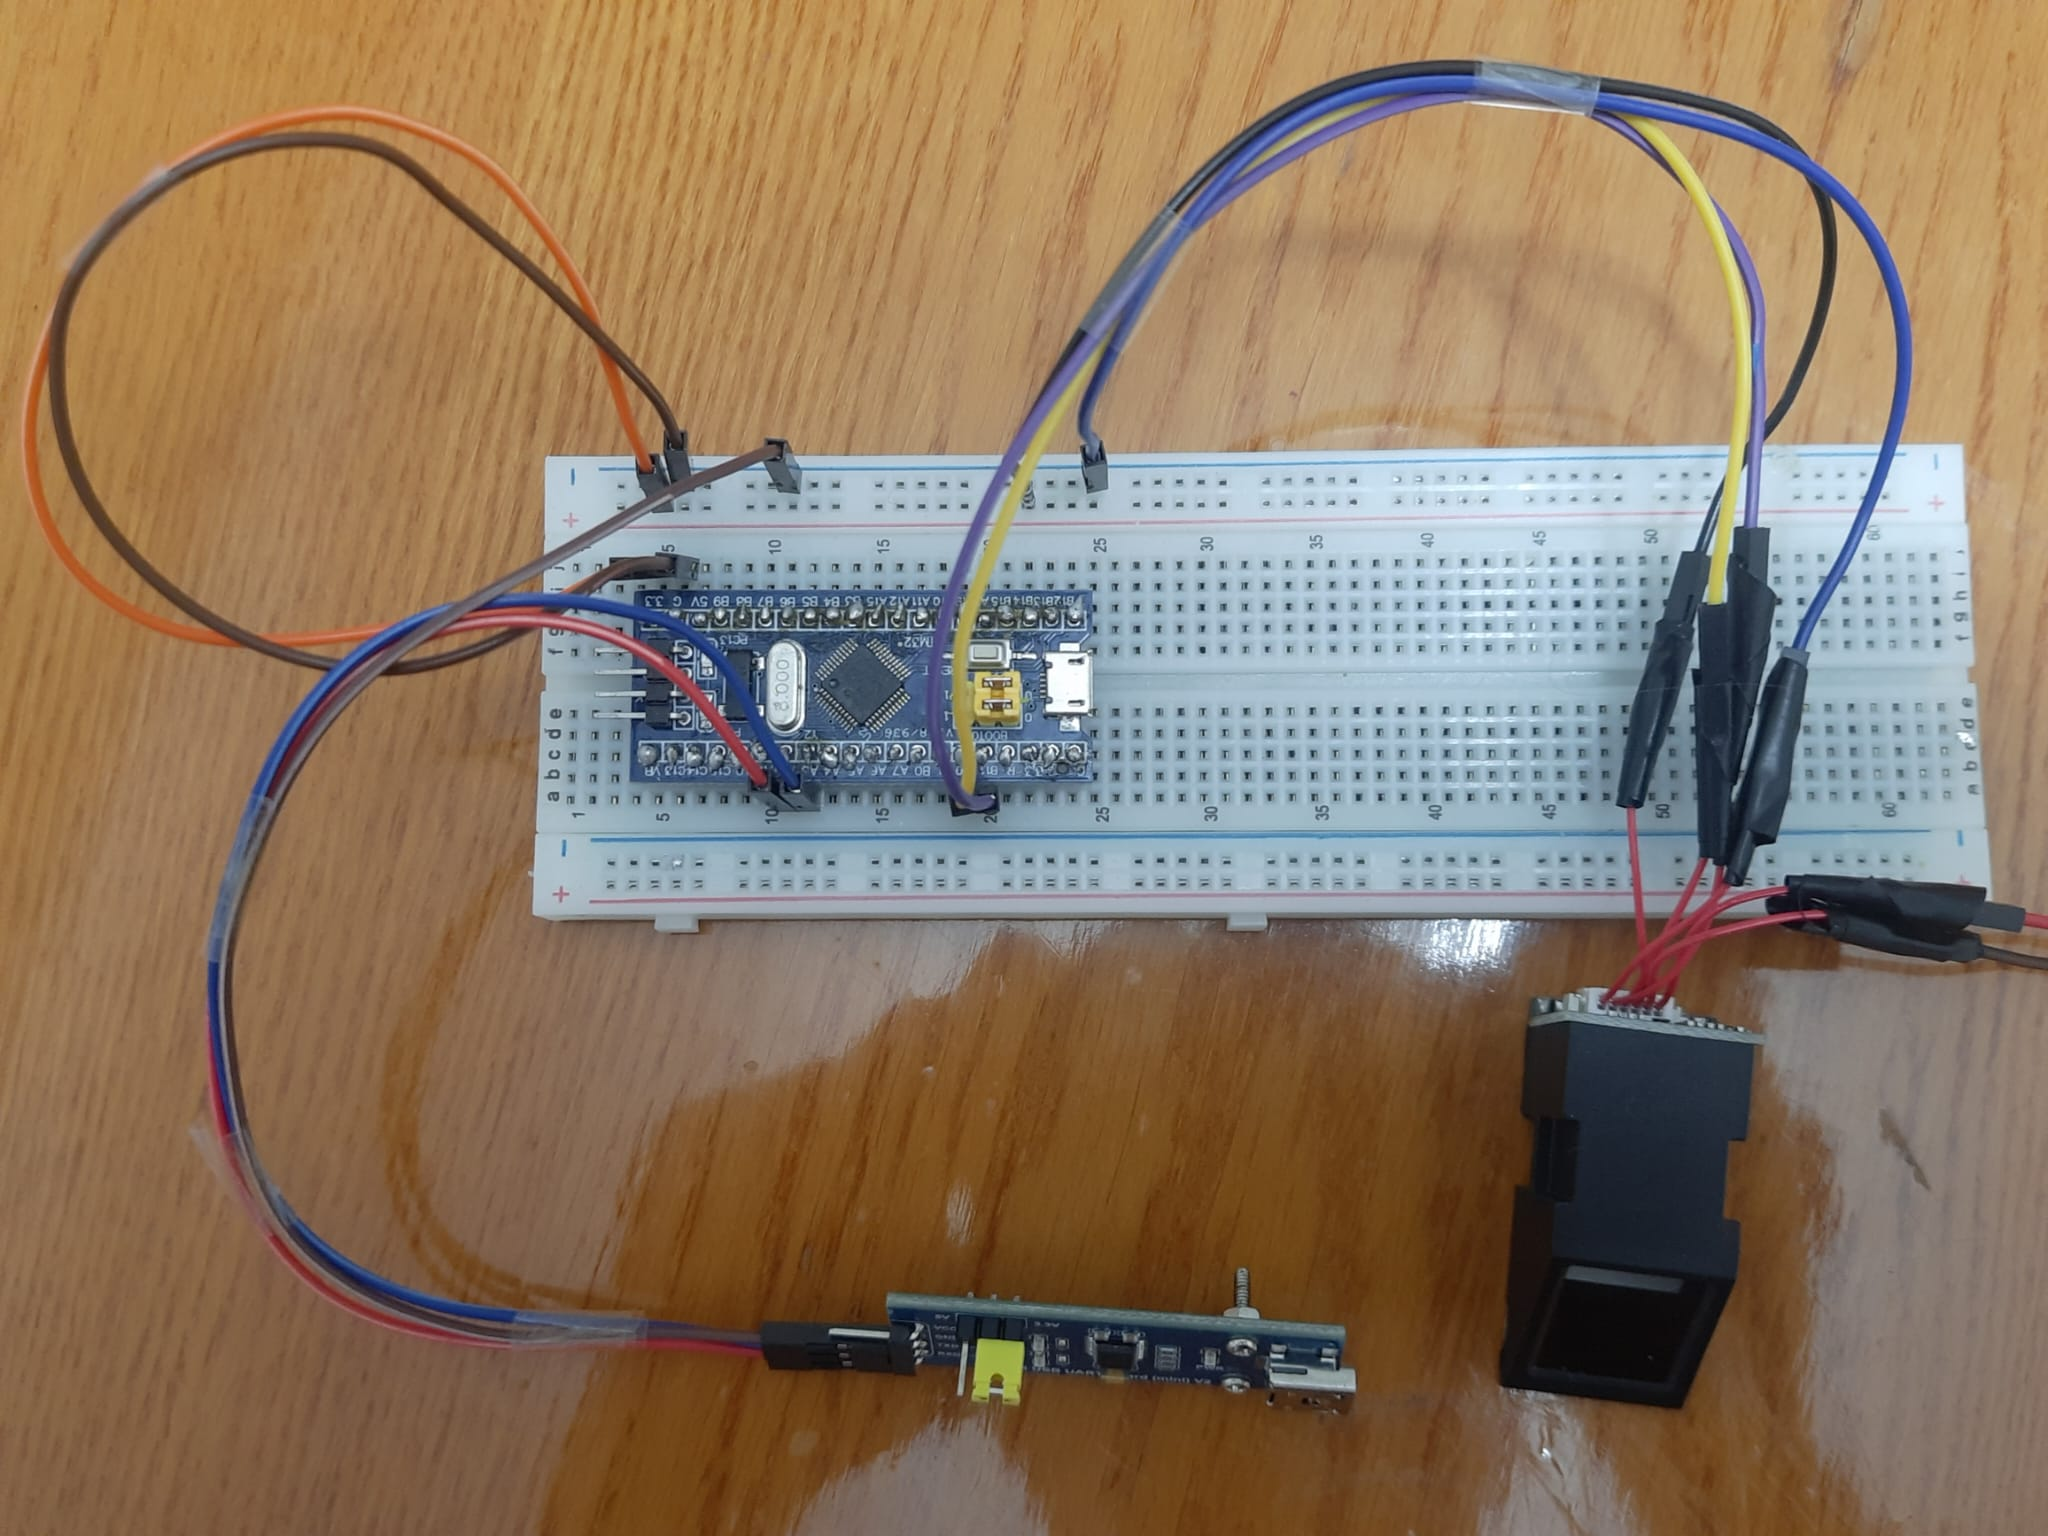
\includegraphics[width=\textwidth]{circuit.jpeg}\\[0.2cm]
        \small Prototype view 1
    \end{minipage}
    \hfill
    \begin{minipage}[t]{0.48\textwidth}
        \centering
        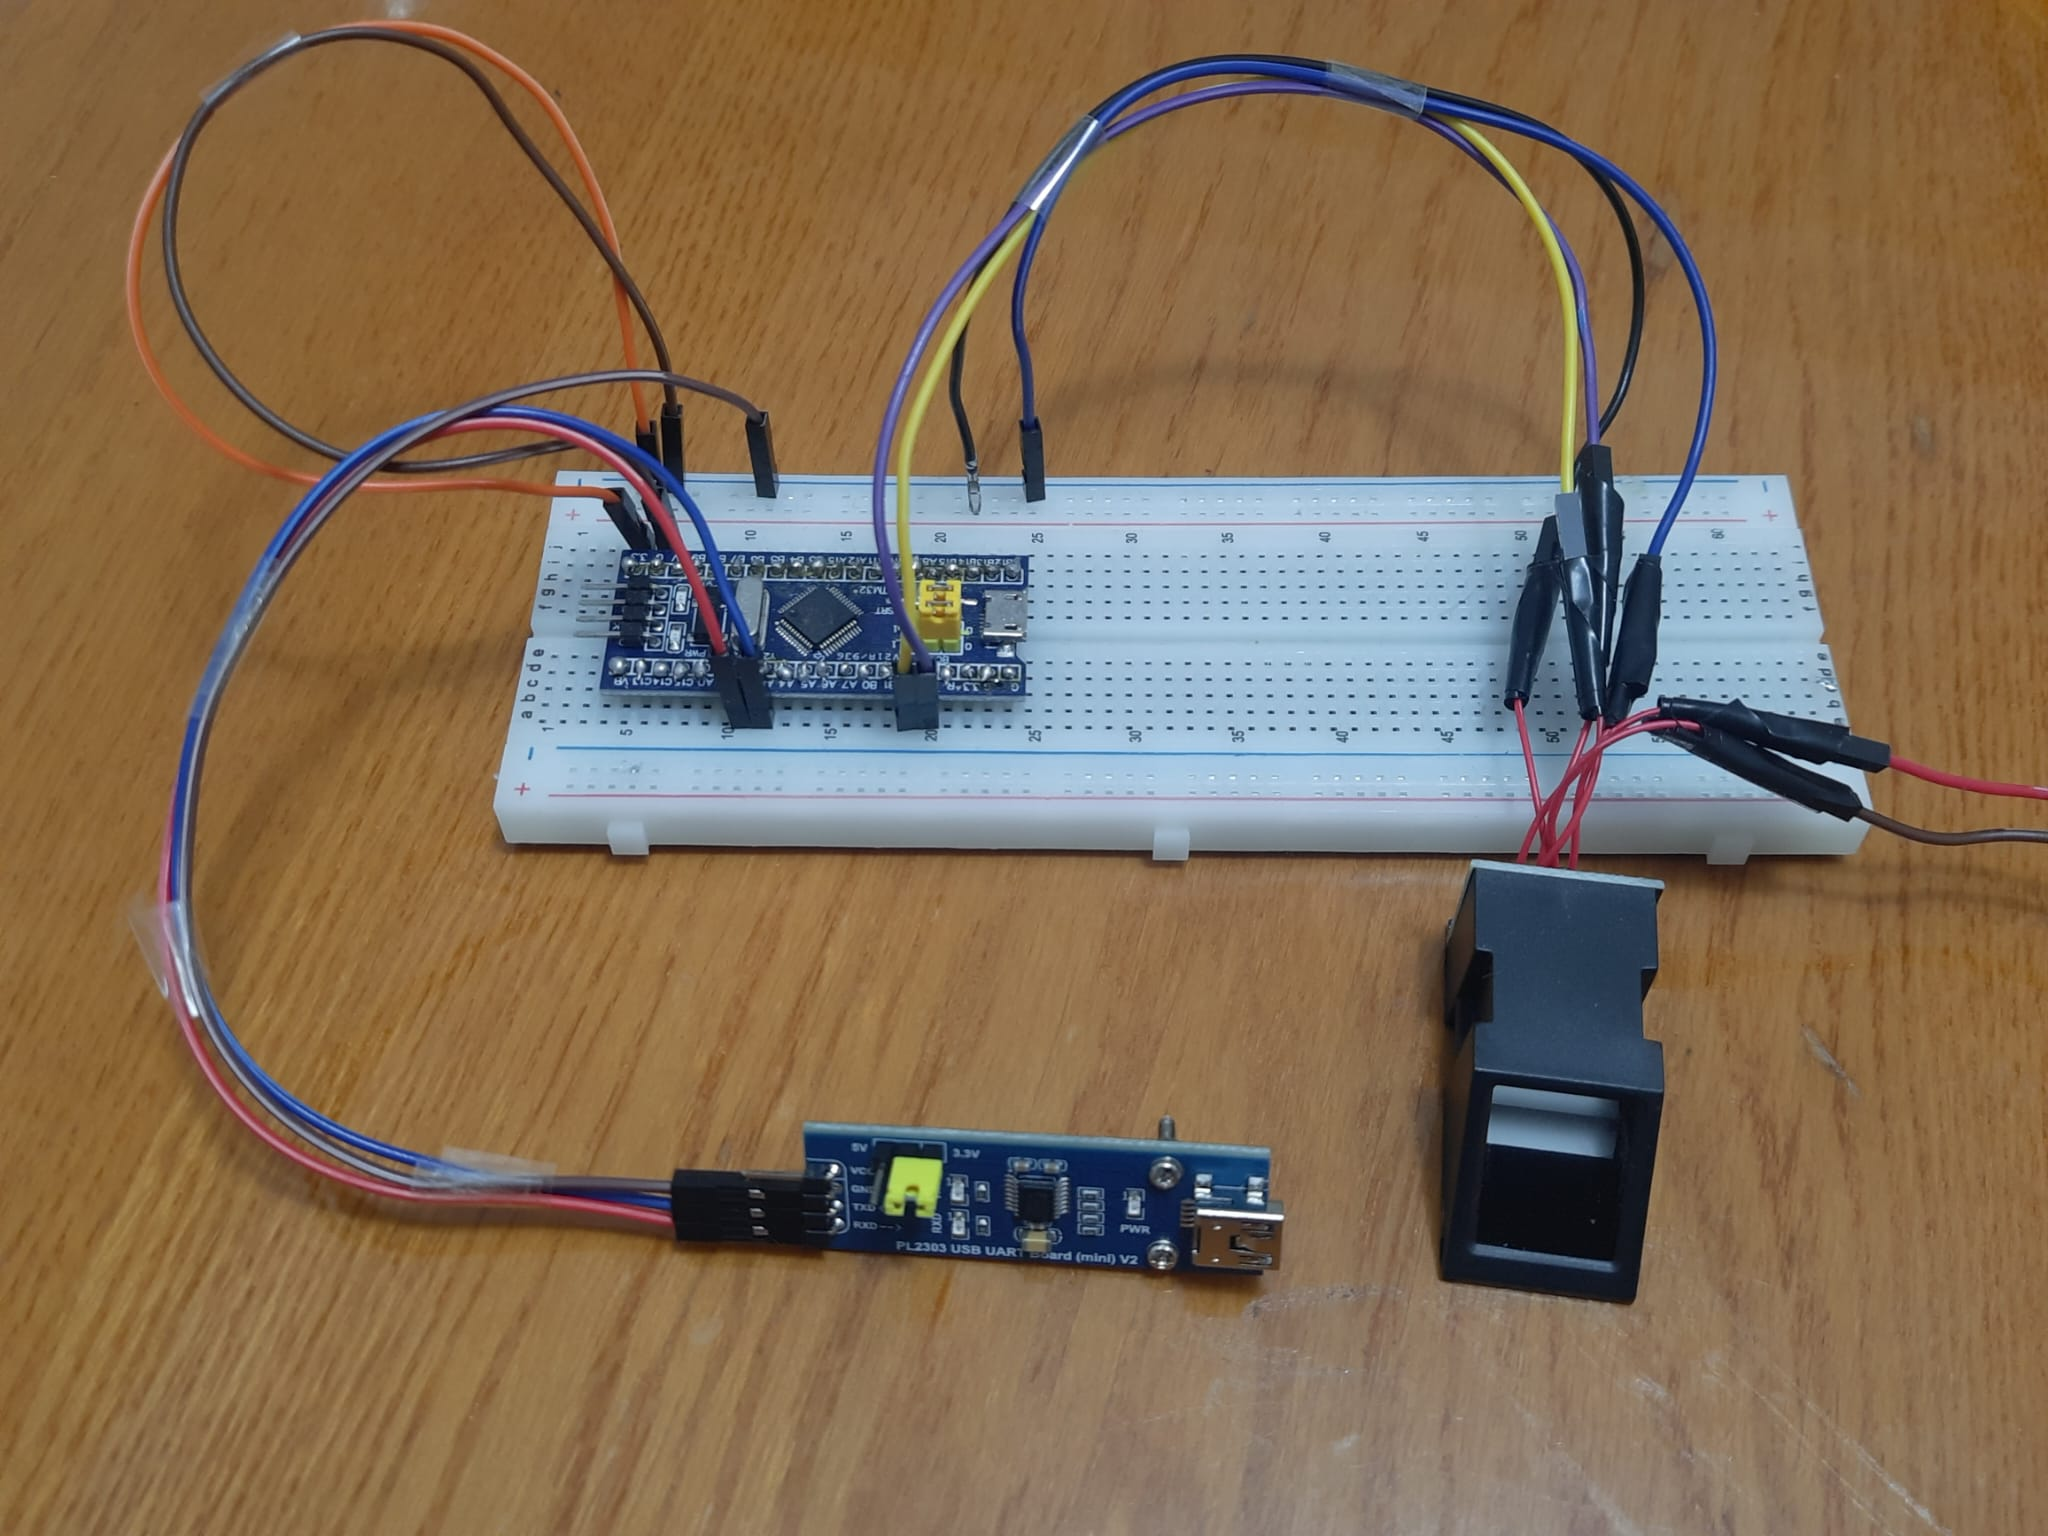
\includegraphics[width=\textwidth]{circuit2.jpeg}\\[0.2cm]
        \small Prototype view 2
    \end{minipage}
    \caption{\label{fig:physical-prototype}Physical prototype including the AS608 fingerprint sensor, STM32 Blue Pill, and PL2303 USB-UART bridge.}
\end{figure}

\section{Host Application}

The host application creates a single controller instance \texttt{vaultController}. As a result, GUI can request high-level actions such as creating a vault, unlocking, locking, force-locking, creating a virtual container, or deleting a vault without knowing the low-level command sequence.

The controller stores the current runtime state of the application. Examples include the selected device, lock status, setup progress, sensor status, registered vault list, security logs, and fingerprint workflow state. These values are exposed as Qt properties, so the interface can update automatically when the state changes.

Long operations are handled asynchronously. Formatting a device, opening a vault, closing a mapper, creating a loop device, or deleting a vault may take time and may fail. For this reason, the controller uses busy flags, completion signals, and recovery paths instead of assuming that every operation finishes immediately.

\section{Firmware Communication}

The host communicates with the STM32 firmware through the \texttt{SerialBridge} class. This bridge opens the selected serial port, configures it at 115200 baud, sends compact binary packets, and parses responses from the firmware. The supported command types include enrollment, verification, deletion, cancellation, key request, and enrolled-fingerprint listing.

The serial layer allows only one fingerprint operation to be active at a time. Enrollment, verification, and key request all depend on sensor state and user interaction, so overlapping them would let the controller receive a response that belongs to the wrong workflow.

Firmware responses are converted into higher-level Qt signals such as verification completed, enrollment completed, key received, operation rejected, or connection lost. The controller then decides how each result should affect the active workflow.

\section{Vault Manager}

The \texttt{vault\_manager} program is a separate command-line component because storage operations require privileges. It prepares the encrypted vault container, opens the decrypted device mapping, creates the ext4 filesystem, mounts and unmounts the vault, creates loop devices, detaches virtual containers, and deletes vault metadata when needed.

On Linux, LUKS containers are commonly managed through the \texttt{cryptsetup} tool. In this project, the vault manager starts \texttt{cryptsetup} as a child process and sends the key through a pipe connected to its standard input. The key is therefore not placed in the command-line arguments, which avoids exposing it in the process list. After the operation finishes, the key buffer is wiped from memory. Listing~\ref{lst:key-stdin} shows a simplified version of this handling.

\begin{lstlisting}[caption={Simplified key handling: the vault key is piped to \texttt{cryptsetup} through standard input and the buffer is cleared after use.},label=lst:key-stdin]
int pipefd[2];
pipe(pipefd);

pid_t pid = fork();
if (pid == 0) {                 /* child: replace stdin with the pipe */
    dup2(pipefd[0], STDIN_FILENO);
    close(pipefd[1]);
    execlp("cryptsetup", "cryptsetup", "luksOpen",
           device, mapper_name, "--key-file=-", (char *)NULL);
    _exit(127);                 /* reached only if exec fails */
}

/* parent: write the 32-byte key, then wipe it */
close(pipefd[0]);
write(pipefd[1], key, key_len);
close(pipefd[1]);
explicit_bzero(key, key_len);   /* clear key buffer after use */
\end{lstlisting}

The same pattern is reused for vault setup, where \texttt{cryptsetup luksFormat} receives the key on standard input instead of as an argument. Passing \texttt{--key-file=-} keeps the secret out of both the argument list and any shell history.

The vault manager also includes cleanup-oriented commands. Normal locking unmounts the filesystem and closes the mapper. Force-lock handles busy mount points by verifying that the mount belongs to the vault before stopping holder processes. Reconciliation is used to clean up leftover mapper or mount state after abnormal situations.

\section{Runtime Recovery}

Several parts of the implementation are written around the possibility of partial failure. A vault may be formatted but not mounted, a mapper may remain open after an interrupted setup, or a mounted filesystem may become busy. An early version of the prototype made this concrete: when a mount failed, the dm-crypt mapper was sometimes left open, and the next unlock attempt then failed with a ``device already exists'' error until the mapper was closed by hand. That bug is the reason the controller and vault manager now distinguish between clean, mapper-only, mounted, busy, and missing-device states instead of a single locked/unlocked flag.

Emergency closing is also connected to application shutdown and abnormal events. If the application exits while the vault is open, or if the runtime state becomes unsafe, the controller attempts to close the vault through the vault manager. This implementation detail supports the design goal of avoiding unstable intermediate states.

Overall, the implementation follows the design principle of keeping responsibilities separate: QML handles interaction, the controller handles workflow state, the serial bridge handles firmware communication, and the vault manager handles storage operations.
